\documentclass{beamer}

\mode<presentation>
{
  \usetheme{default}
  \usecolortheme{default}
  \usefonttheme{default}
  \setbeamertemplate{navigation symbols}{}
  \setbeamertemplate{caption}[numbered]
  \setbeamertemplate{footline}[page number]
  \setbeamercolor{frametitle}{fg=white}
  \setbeamercolor{footline}{fg=black}
} 

\usepackage[english]{babel}
\usepackage[utf8x]{inputenc}
\usepackage{tikz}
\usepackage{listings}
\usepackage{courier}
\usepackage{array}
\usepackage{bold-extra}
\usepackage{minted}

\xdefinecolor{darkblue}{rgb}{0.1,0.1,0.7}
\xdefinecolor{darkgreen}{rgb}{0,0.5,0}
\xdefinecolor{darkgrey}{rgb}{0.35,0.35,0.35}
\xdefinecolor{darkorange}{rgb}{0.8,0.5,0}
\xdefinecolor{darkred}{rgb}{0.7,0,0}
\xdefinecolor{dianablue}{rgb}{0.18,0.24,0.31}
\definecolor{commentgreen}{rgb}{0,0.6,0}
\definecolor{stringmauve}{rgb}{0.58,0,0.82}

\lstset{ %
  backgroundcolor=\color{white},      % choose the background color
  basicstyle=\ttfamily\small,         % size of fonts used for the code
  breaklines=true,                    % automatic line breaking only at whitespace
  captionpos=b,                       % sets the caption-position to bottom
  commentstyle=\color{commentgreen},  % comment style
  escapeinside={\%*}{*)},             % if you want to add LaTeX within your code
  keywordstyle=\color{blue},          % keyword style
  stringstyle=\color{stringmauve},    % string literal style
  showstringspaces=false,
  showlines=true
}

\lstdefinelanguage{scala}{
  morekeywords={abstract,case,catch,class,def,%
    do,else,extends,false,final,finally,%
    for,if,implicit,import,match,mixin,%
    new,null,object,override,package,%
    private,protected,requires,return,sealed,%
    super,this,throw,trait,true,try,%
    type,val,var,while,with,yield},
  otherkeywords={=>,<-,<\%,<:,>:,\#,@},
  sensitive=true,
  morecomment=[l]{//},
  morecomment=[n]{/*}{*/},
  morestring=[b]",
  morestring=[b]',
  morestring=[b]"""
}

\title[2017-09-05-nanoaod-xpog]{Performance studies on NanoAOD}
\author{Jim Pivarski}
\institute{Princeton University -- DIANA}
\date{September 5, 2017}

\begin{document}

\logo{\pgfputat{\pgfxy(0.11, 8)}{\pgfbox[right,base]{\tikz{\filldraw[fill=dianablue, draw=none] (0 cm, 0 cm) rectangle (50 cm, 1 cm);}}}\pgfputat{\pgfxy(0.11, -0.6)}{\pgfbox[right,base]{\tikz{\filldraw[fill=dianablue, draw=none] (0 cm, 0 cm) rectangle (50 cm, 1 cm);}
\includegraphics[height=0.99 cm]{diana-hep-logo.png}\tikz{\filldraw[fill=dianablue, draw=none] (0 cm, 0 cm) rectangle (4.9 cm, 1 cm);}}}}

\begin{frame}
  \titlepage
\end{frame}

\logo{\pgfputat{\pgfxy(0.11, 8)}{\pgfbox[right,base]{\tikz{\filldraw[fill=dianablue, draw=none] (0 cm, 0 cm) rectangle (50 cm, 1 cm);}
\includegraphics[height=1 cm]{diana-hep-logo.png}}}}

% Uncomment these lines for an automatically generated outline.
%\begin{frame}{Outline}
%  \tableofcontents
%\end{frame}

%%%%%%%%%%%%%%%%%%%%%%%%%%%%%%%%%%%%%%%%%%%%%%%%%%%%%%%

\begin{frame}{Why I'm interested}
\vspace{0.5 cm}
NanoAOD could be the first standardized data format (across a whole experiment) that is simple enough to directly import into industry-standard tools--- Pandas, Spark, machine learning, etc.

\vspace{0.3 cm}
\begin{itemize}\setlength{\itemsep}{0.5 cm}
\item<2-> We can read complex formats (e.g.\ MiniAOD) in these frameworks by directly translating the TBranch structure, but this structure is intended to fill classes, not to be understood by data analysts.

\item<3-> We can also read custom formats generated by each analysis group (e.g.\ reduced TNtuples), but each of these has a limited user base.
\end{itemize}

\vspace{0.2 cm}
\uncover<4->{NanoAOD is a good candidate for a centralized analysis service.}
\end{frame}

\begin{frame}{Real-world test of BulkIO}
\vspace{0.5 cm}
BulkIO is a new ROOT feature (expected ROOT 6.12) that exposes purely numerical TBasket data as arrays without any copying or method calls in the loop over events.

\vspace{0.5 cm}
In the same ROOT version, I'm adding a PyROOT extension to drop these data into Numpy arrays.

35$\times$ faster (on uncompressed data in warm cache)

\end{frame}

\begin{frame}{File size}
\begin{center}
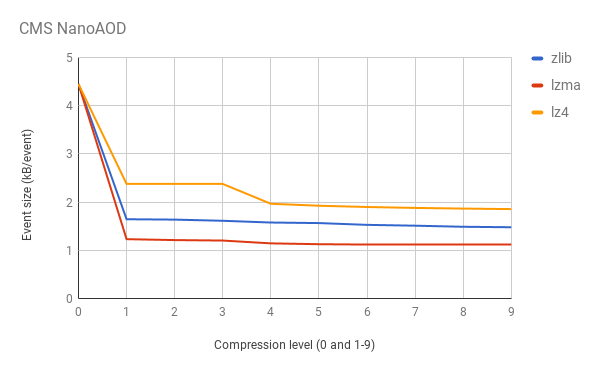
\includegraphics[width=\linewidth]{size-vs-compression.png}
\end{center}

LZMA provides the best compression; LZ4 is within a factor of 2.
\vspace{\baselineskip}
\end{frame}

\begin{frame}{Write throughput}
\begin{center}
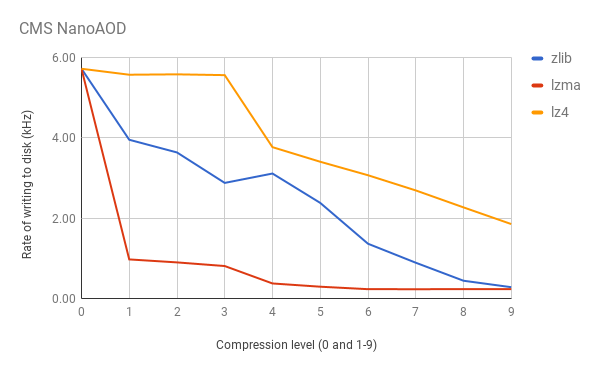
\includegraphics[width=\linewidth]{write-vs-compression.png}
\end{center}

LZ4 levels 1--3 have no overhead relative to {\tt TTree::CopyTree}.
\vspace{\baselineskip}
\end{frame}

\begin{frame}{Read throughput (MakeClass)}
\begin{center}
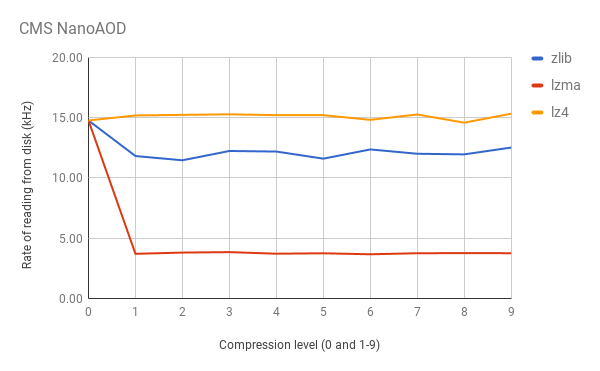
\includegraphics[width=\linewidth]{read-vs-compression.png}
\end{center}

All LZ4 levels have no overhead relative to reading data into a class generated by MakeClass. LZ4 is 4 times faster to read then LZMA.
\end{frame}

\begin{frame}{Read throughput (BulkIO: note the axis!)}
\begin{center}
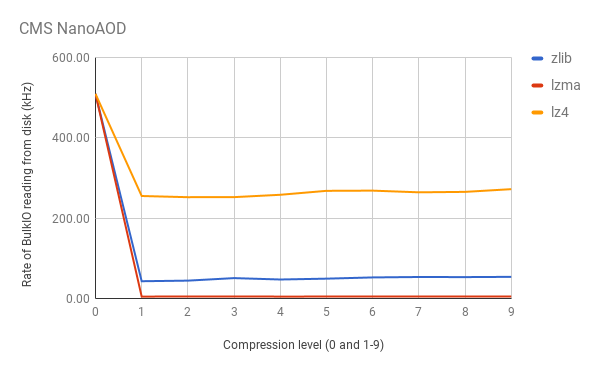
\includegraphics[width=\linewidth]{bulk-vs-compression.png}
\end{center}

BulkIO reads uncompressed data 35 times faster than filling a class; LZ4 drops this to 17 times. LZMA is 50 times slower than LZ4.
\end{frame}

\begin{frame}{View all as scatter plots: top-left is best}
\vspace{0.5 cm}
\begin{columns}
\column{0.4\linewidth}
\mbox{ } \hfill write vs size \hfill \mbox{ }

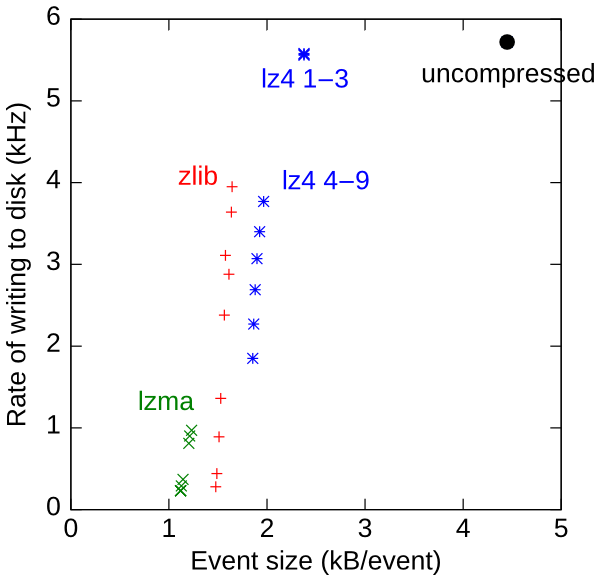
\includegraphics[width=\linewidth]{write.png}
\vspace{3 cm}
\column{0.4\linewidth}
\mbox{ } \hfill read vs size \hfill \mbox{ }

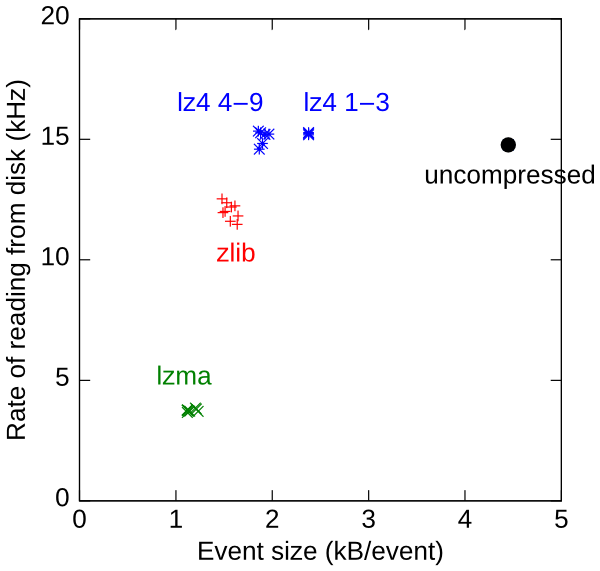
\includegraphics[width=\linewidth]{read.png}
\column{0.4\linewidth}
\vspace{3 cm}

\mbox{ } \hfill BulkIO vs size \hfill \mbox{ }

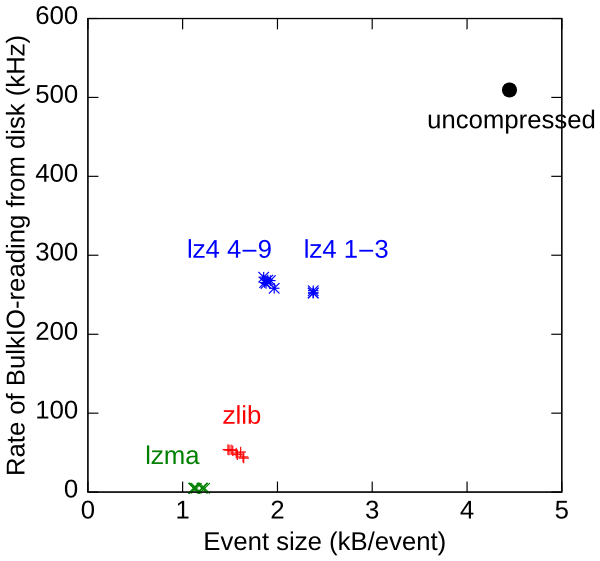
\includegraphics[width=\linewidth]{bulk.png}
\end{columns}

\vspace{-2\baselineskip}
It's about trade-offs, but the cost of \\ LZMA for BulkIO is very high!
\end{frame}




\end{document}
